\label{section:quality}
L'intégration avec Jenkins nous a permis de valider l'intégrité du projet au fur et à mesure que nous développions. Les tests unitaires étaient en effet effectués automatiquement.......... \\
Pour réaliser la mesure de métriques de qualité du projet, nous avons utilisé un plugin d'intellij nommé CodeMR, qui génère automatiquement un rapport contenant les résultats d'un grand nombre de métriques de qualité selon plusieurs critères. 
\\ Les fichiers html générés sont placés automatiquement dans le sous-dossier \path{/codemr/Ludotheque/html}
\footnote{Rapport qualité : \url{https://github.com/victorsmits/Ludotheque/tree/master/codemr/Ludotheque/html/main_report}}.

\subsection{Taille}
    \begin{figure}[h!]
        \centering
        \subfloat[Ancienne taille.]{{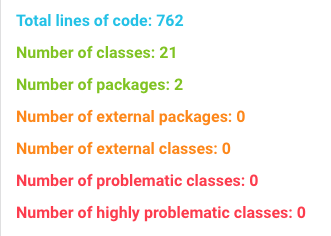
\includegraphics[width=0.45\textwidth]{Figures/Old_Size.png}}}
        \qquad
        \subfloat[Nouvelle taille.]{{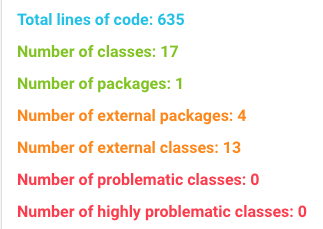
\includegraphics[width=0.45\textwidth]{Figures/New_Size.png}}}
        \caption{Taille du projet.}
    \end{figure}
La taille du code a diminué de manière non négligeable; diminution de 16\% du nombre de lignes de code, expliquée principalement par la suppression de nombreuses duplications de code ; et diminution de 19\% du nombre de classes dans le projet, expliqué par la suppression de plusieurs classes entièrement redondantes et non implémentées. 
\paragraph{}
La diminution de la taille du code pour une même qualité globale entraîne souvent une meilleure lisibilité du code, et donc une augmentation de sa maintenabilité. 
\newpage
\subsection{Complexité}

    \begin{figure}[h!]
        \centering
        \subfloat[Ancienne Complexité interne.]{{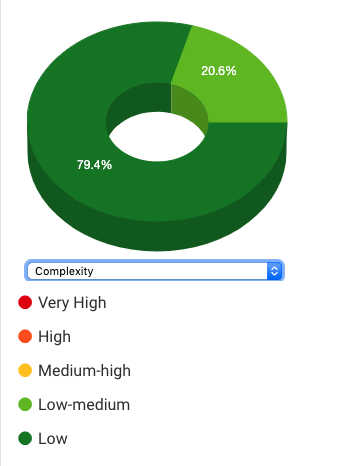
\includegraphics[width=0.47\textwidth]{Figures/Old_Complex.png}}}
        \qquad
        \subfloat[Nouvelle complexité interne.]{{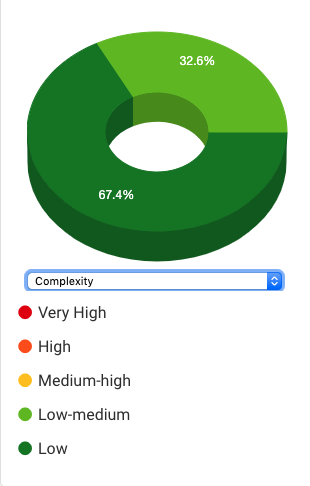
\includegraphics[width=0.4\textwidth]{Figures/New_Complex.png}}}
        \caption{Complexité générale.}
    \end{figure}
On constate que la complexité du projet a augmenté avec nos modifications, donc que la qualité du projet a décru en ce qui concerne la maintenabilité; ceci est probablement expliqué par le fait que nous avons implémenté plusieurs classes et méthodes qui étaient laissées vides par l'équipe précédente, nous avons notamment fait augmenter les indices de McCabe, les interactions entre les classes, etc. Les valeurs de métriques de complexité du projet tel que nous l'avons reçu ne sont donc pas représentatives de la complexité réelle du design initial. 

\newpage
\subsection{Cohésion}
    \begin{figure}[h!]
        \centering
        \subfloat[Ancien manque de cohésion interne.]{{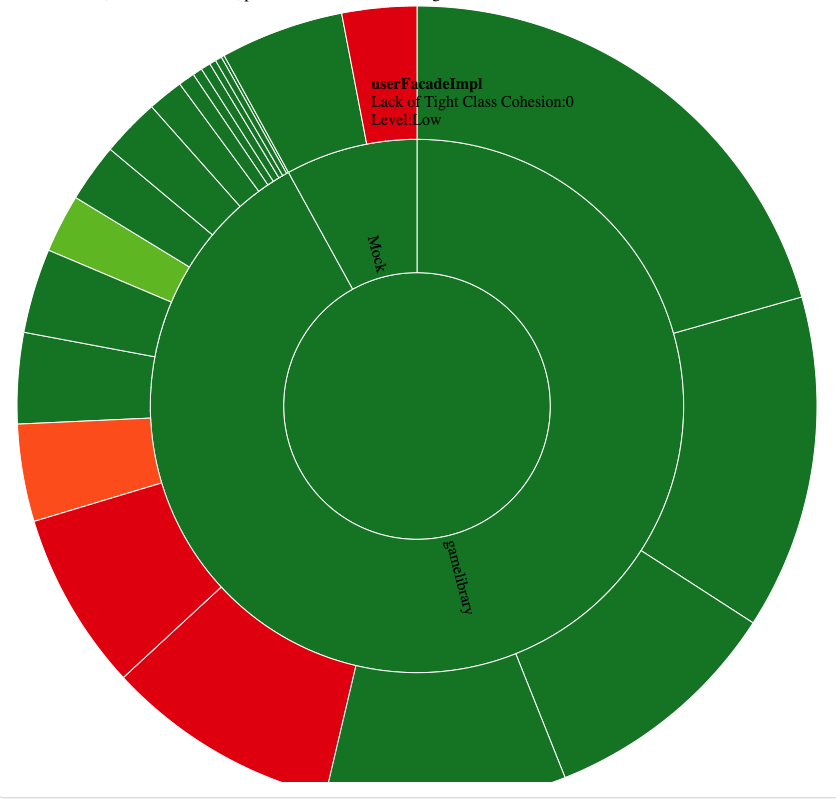
\includegraphics[width=0.45\textwidth]{Figures/Old_Cohesion.png}}}
        \qquad
        \subfloat[Nouveau manque de cohésion interne.]{{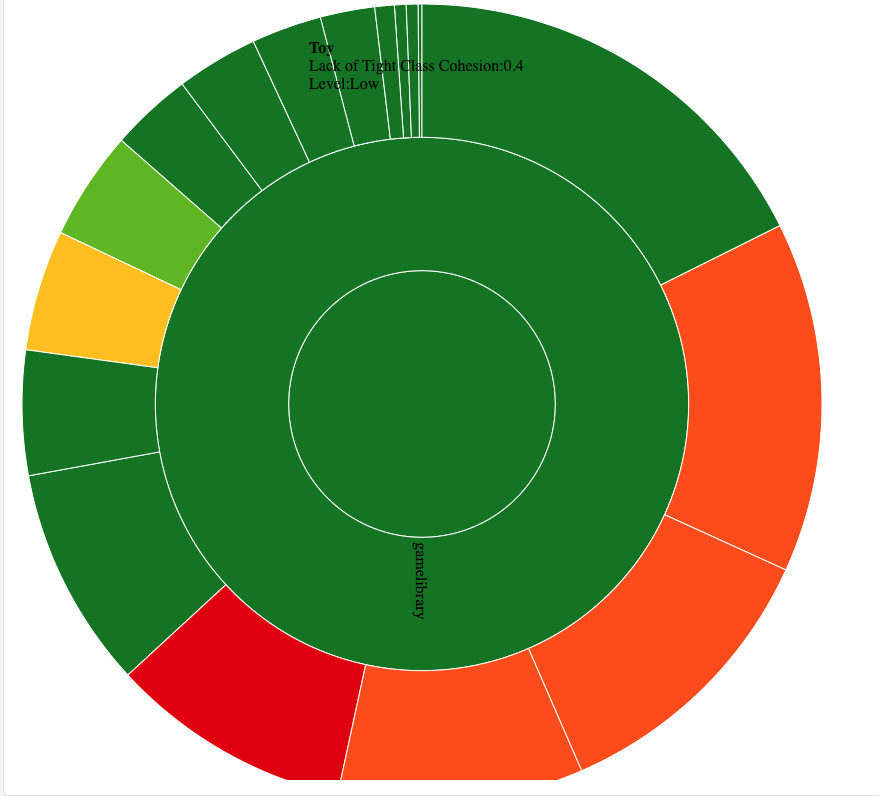
\includegraphics[width=0.45\textwidth]{Figures/New_Cohesion.png}}}
        \caption{Manque de cohésion. Chaque portion de disque représente une classe du projet; sa couleur, le taux de manque de cohésion.}
    \end{figure}
    \begin{figure}[h!]
        \centering
        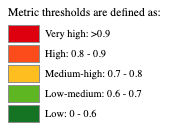
\includegraphics{Figures/Legend.png}
        \caption{Légende}
    \end{figure}
Ce paramètre décrit la qualité des relations à l'intérieur d'une classe (utilisation de tous les attributs par les méthodes de la classe donc pas d'attribut inutile, par exemple); une cohésion élevée (donc vert, manque de cohésion bas) est associé avec des qualités telles que la robustesse et la maintenabilité. En modifiant le code, nous avons globalement amélioré la cohésion du programme, même si certaines classes telles que Person ou Authentification se sont dégradées, ce qui s'explique par le fait que nous avons ajouté de nombreuses méthodes à cette classe.  

\newpage
\subsection{Couplage}
    \begin{figure}[h!]
        \centering
        \subfloat[Ancien couplage interne.]{{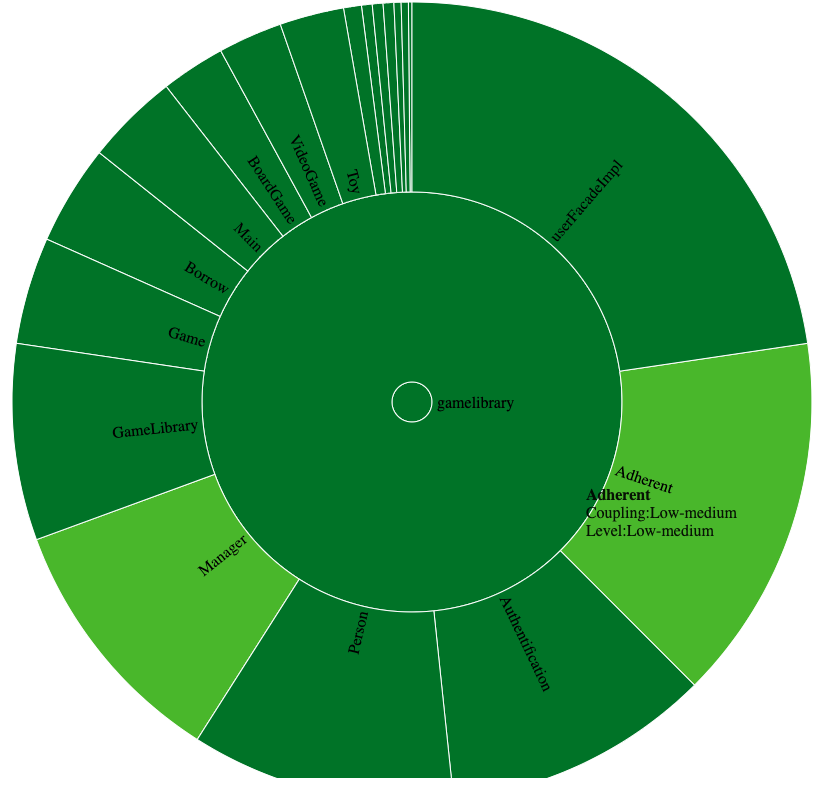
\includegraphics[width=0.45\textwidth]{Figures/Old_Coupling.png}}}
        \qquad
        \subfloat[Nouveau couplage interne.]{{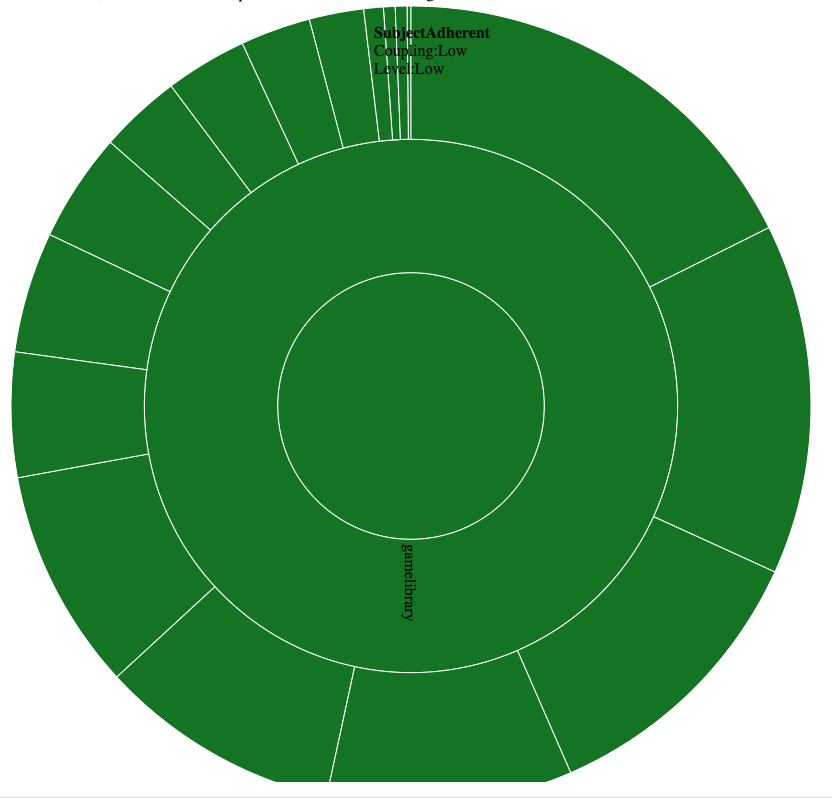
\includegraphics[width=0.45\textwidth]{Figures/New_Coupling.png}}}
        \caption{Couplage interne.}
        \label{fig:couplage_interne}
    \end{figure}
    \begin{figure}[h!]
        \centering
        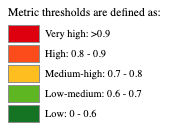
\includegraphics{Figures/Legend.png}
        \caption{Légende}
    \end{figure}
    \paragraph{}
    Nous pouvons constater que le couplage entre les classes a légèrement diminué \footnote{Le couplage des classes Adherent et Manager a diminué}. Cependant, puisque nous n'avons presque pas changé la structure du programme, il semble logique que le couplage entre les classes n'ait presque pas changé. Ce couplage relativement bas implique que le projet devrait être facilement extensible.

\newpage
\subsection{Erreur de Style}
    \begin{figure}[h!]
        \centering
        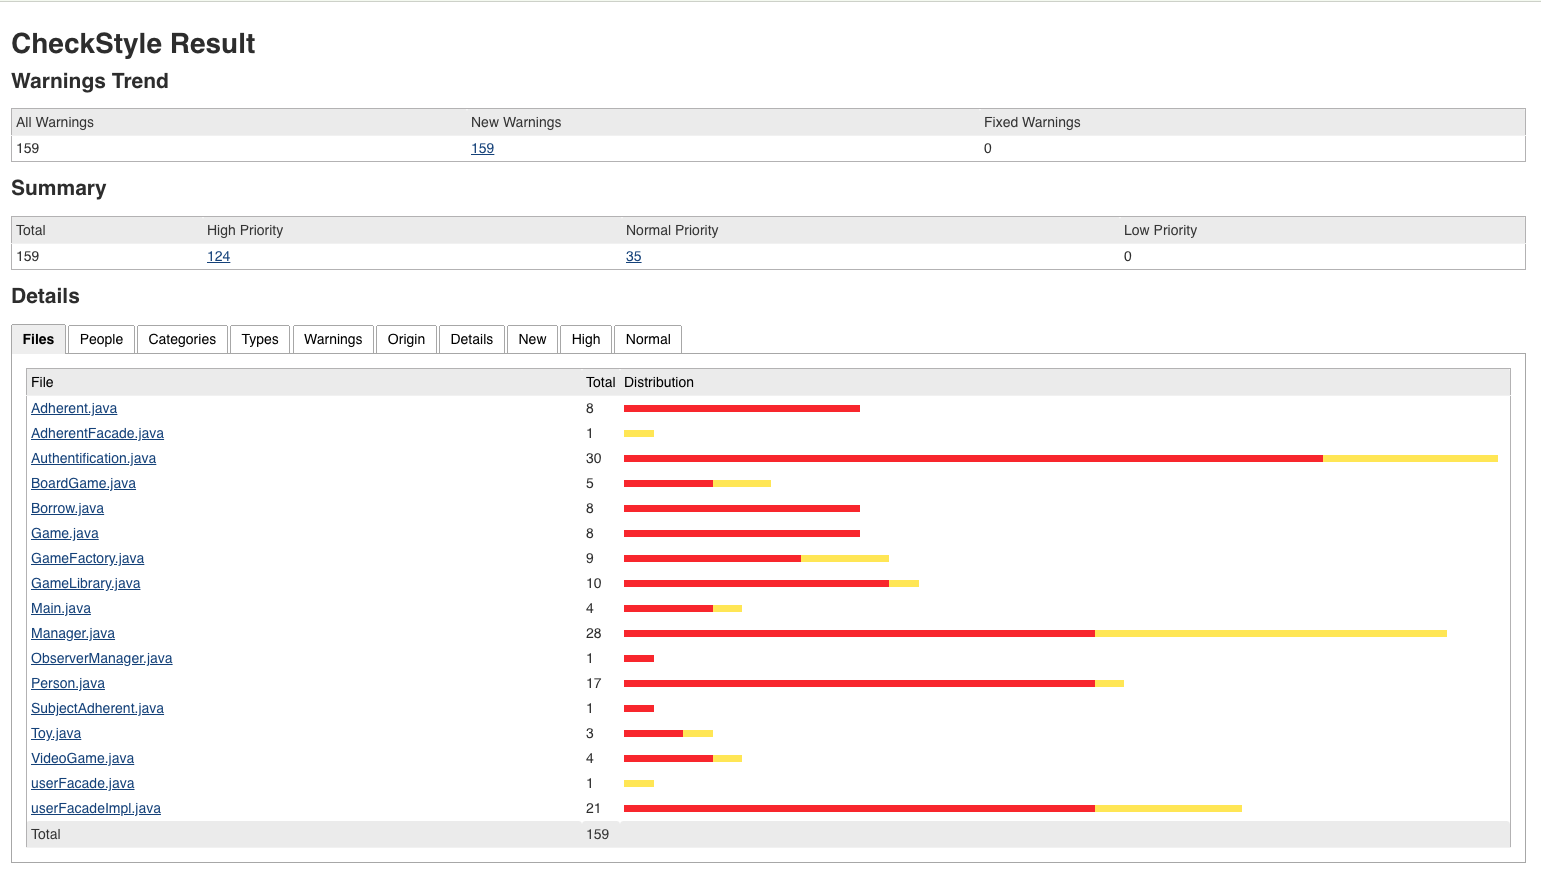
\includegraphics[width=0.8\textwidth]{Figures/Old_CheckStyle.png}
        \caption{Ancienne erreur de style.}
        \label{fig:checkstyle}
    \end{figure}
    
    \paragraph{}
    Comme nous pouvons le voire dans la figure \ref{fig:checkstyle} la première version du code contenait de nombreuse erreur de style de code.
    Nous avons donc résolut toutes les erreurs de check Style qui ont été repérée par Jenkins via la comparaison aux règles de codage de Google.